\documentclass{article}
\usepackage{karnaugh-map}
\usepackage[hyphens]{url}

\begin{document}

\title{Design of a BCD–to–Seven-Segment Decoder Universitas Diponegoro }
\author{}
\date{}

\maketitle

\section{Kelompok D}

\begin{itemize}
    \item Muchammad Yuda Tri Ananda (24060124110142)
    \item Muhammad Alfaiq Rido Salafy (24060124140148)
    \item Naufal Rayan Attallah (24060124140148)
\end{itemize}

\section{Spesifikasi}

Banyak produk elektronik konsumen seperti jam alarm menggunakan tampilan digital berbasis dioda pemancar cahaya (LED). Setiap digit pada tampilan terbentuk dari tujuh segmen LED, di mana masing-masing segmen dapat menyala melalui sinyal digital. 

Decoder BCD-ke-seven-segment adalah rangkaian kombinasi yang menerima digit desimal dalam bentuk BCD dan menghasilkan keluaran yang tepat untuk segmen-segmen tampilan sesuai dengan digit desimal tersebut. Terdapat tujuh keluaran dari decoder (a, b, c, d, e, f, g) yang akan mengendalikan segmen terkait pada tampilan, seperti yang terlihat pada Gambar 3-38(a). Penomoran untuk setiap digit desimal ditunjukkan pada Gambar 3-38(b).

Decoder BCD-ke-seven-segment ini memiliki empat masukan (A, B, C, D) untuk digit BCD dan tujuh keluaran (a sampai g) untuk mengendalikan segmen tampilan.

\section{Formulasi}

Tabel kebenaran untuk rangkaian kombinasi ini tercantum pada Tabel 3-9. Berdasarkan Gambar 3-38(b), setiap digit BCD akan menyalakan segmen-segmen yang sesuai untuk tampilan desimal. Sebagai contoh, BCD 0011 merepresentasikan digit desimal 3, yang akan menyalakan segmen a, b, c, d, dan g.

Tabel kebenaran ini mengasumsikan bahwa sinyal logika 1 menyalakan segmen dan sinyal logika 0 mematikan segmen. Beberapa tampilan seven-segment bekerja sebaliknya, di mana segmen menyala dengan sinyal logika 0. Dalam kasus ini, keluaran dari decoder harus dikomplemenkan.

Kombinasi biner 1010 hingga 1111 tidak memiliki arti dalam BCD. Dalam contoh sebelumnya, kita mengasumsikan kombinasi tersebut sebagai kondisi don't-care. Dengan pendekatan ini, desain kemungkinan akan menghasilkan tampilan acak dan tidak bermakna untuk kombinasi masukan yang tidak digunakan. 

Namun, pendekatan yang lebih aman adalah mematikan semua segmen ketika salah satu kombinasi masukan yang tidak digunakan terjadi, untuk menghindari tampilan yang tidak diinginkan. Meskipun pendekatan ini meningkatkan kompleksitas rangkaian, hal tersebut lebih andal.

\begin{figure}[h!]
    \centering
    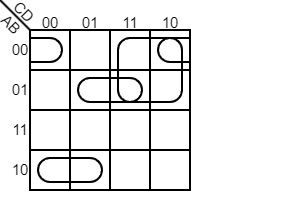
\includegraphics[width=1\linewidth]{image.png}
    \caption{Tampilan BCD ke Seven-Segment}
    \label{fig:display-bcd-seven-segment}
\end{figure}

\begin{table}[h!]
\centering
\begin{tabular}{|c|c|c|c|c|c|c|c|c|c|c|}
\hline
\multicolumn{4}{|c|}{\textbf{BCD Input}} & \multicolumn{7}{c|}{\textbf{Seven-Segment Decoder}} \\ 
\hline
A & B & C & D & a & b & c & d & e & f & g \\
\hline
0 & 0 & 0 & 0 & 1 & 1 & 1 & 1 & 1 & 1 & 0 \\
0 & 0 & 0 & 1 & 0 & 1 & 1 & 0 & 0 & 0 & 0 \\
0 & 0 & 1 & 0 & 1 & 1 & 0 & 1 & 1 & 0 & 1 \\
0 & 0 & 1 & 1 & 1 & 1 & 1 & 1 & 0 & 0 & 1 \\
0 & 1 & 0 & 0 & 0 & 1 & 1 & 0 & 0 & 1 & 1 \\
0 & 1 & 0 & 1 & 1 & 0 & 1 & 1 & 0 & 1 & 1 \\
0 & 1 & 1 & 0 & 1 & 0 & 1 & 1 & 1 & 1 & 1 \\
0 & 1 & 1 & 1 & 1 & 1 & 1 & 0 & 0 & 0 & 0 \\
1 & 0 & 0 & 0 & 1 & 1 & 1 & 1 & 1 & 1 & 1 \\
1 & 0 & 0 & 1 & 1 & 1 & 1 & 1 & 0 & 1 & 1 \\
\hline
\multicolumn{4}{|c|}{Masukan lainnya} & 0 & 0 & 0 & 0 & 0 & 0 & 0 \\
\hline
\end{tabular}
\caption{Truth Table for BCD–to–Seven-Segment Decoder}
\end{table}


\pagebreak

\section{Optimisasi}

% ==================================================
\subsection{A. Optimisasi yang a}

\[
a(A, B, C, D) = \Sigma_{m}(0, 2, 3, 5, 6, 7, 8, 9)
\]

\[
\begin{karnaugh-map}[4][4][1][$D$][$C$][$B$][$A$]
    \minterms{0, 2, 3, 5, 6, 7, 8, 9}
    \maxterms{1,4,10,11,12,13,14,15}
    
    \implicant{5}{7}
    \implicant{8}{9}
    \implicant{3}{6}
    
    \implicantedge{0}{0}{2}{2}
\end{karnaugh-map}
\]

\[
\overline{A}\,C\,+\,A\,\overline{B}\,\overline{C}\,+\,\overline{A}\,B\,D\,+\,\overline{A}\,\overline{B}\,\overline{D}
\]

\begin{figure}[h!]
    \centering
    \includegraphics[width=1\linewidth]{Main (8).png}
    \caption{Circuit a}
    \label{fig:enter-label}
\end{figure}

% ==================================================

% ==================================================
\subsection{B. Optimisasi yang b}

\[
b(A, B, C, D) = \Sigma_{m}(0, 1, 2, 3, 4, 7, 8,9)
\]

\[
\begin{karnaugh-map}[4][4][1][$D$][$C$][$B$][$A$]
    \minterms{0, 1, 2, 3, 4, 7, 8, 9}
    \maxterms{5,6,10,11,12,13,14,15}
    
    \implicant{0}{2}
    \implicant{0}{4}
    \implicant{3}{7}
    
    % \implicant{8}{9}
    
    % \implicant{3}{6}
    
    \implicantedge{0}{1}{8}{9}
\end{karnaugh-map}
\]

\[
\overline{A}\,\overline{B}\,+\,\overline{B}\,\overline{C}\,+\,\overline{A}\,C\,D\,+\,\overline{A}\,\overline{C}\,\overline{D}
\]

\begin{figure}[h!]
    \centering
    \includegraphics[width=1\linewidth]{Main (9).png}
    \caption{Circuit b}
    \label{fig:enter-label}
\end{figure}

% ==================================================

\pagebreak

% ==================================================
\subsection{C. Optimisasi yang c}

\[
c(A, B, C, D) = \Sigma_{m}(0, 1, 3, 4, 5, 6, 7, 8, 9)
\]

\[
\begin{karnaugh-map}[4][4][1][$D$][$C$][$B$][$A$]
    \minterms{0, 1, 3, 4, 5, 6, 7, 8, 9}
    \maxterms{2,10,11,12,13,14,15}
    
    \implicant{4}{6}
    \implicant{1}{7}
    % \implicant{3}{7}
    
    % \implicant{8}{9}
    
    % \implicant{3}{6}
    
    \implicantedge{0}{1}{8}{9}
\end{karnaugh-map}
\]

\[
\overline{A}\,B\,+\,\overline{A}\,D\,+\,\overline{B}\,\overline{C}
\]

\begin{figure}[h!]
    \centering
    \includegraphics[width=1\linewidth]{Main (10).png}
    \caption{Circuit c}
    \label{fig:enter-label}
\end{figure}

% ==================================================

\pagebreak

% ==================================================
\subsection{D. Optimisasi yang d}

\[
d(A, B, C, D) = \Sigma_{m}(0, 2, 3, 5, 6, 8, 9)
\]

\[
\begin{karnaugh-map}[4][4][1][$D$][$C$][$B$][$A$]
    \minterms{0, 2, 3, 5, 6, 8, 9}
    \maxterms{1,4,7,10,11,12,13,14,15}
    
    \implicant{3}{2}
    \implicant{2}{6}
    \implicant{5}{5}
    \implicant{8}{9}
    
    % \implicant{8}{9}
    
    % \implicant{3}{6}
    
    \implicantedge{0}{0}{2}{2}
\end{karnaugh-map}
\]

\[
A\,\overline{B}\,\overline{C}\,+\,\overline{A}\,\overline{B}\,C\,+\,\overline{A}\,C\,\overline{D}\,+\,\overline{A}\,\overline{B}\,\overline{D}\,+\,\overline{A}\,B\,\overline{C}\,D
\]

\begin{figure}[h!]
    \centering
    \includegraphics[width=1\linewidth]{Main (16).png}
    \caption{Circuit d}
    \label{fig:enter-label}
\end{figure}
% ==================================================

\pagebreak

% ==================================================
\subsection{E. Optimisasi yang e}

\[
e(A, B, C, D) = \Sigma_{m}(0, 2, 6, 8)
\]

\[
\begin{karnaugh-map}[4][4][1][$D$][$C$][$B$][$A$]
    \minterms{0, 2, 6, 8}
    \maxterms{1,3,4,5,7,9,10,11,12,13,14,15}
    
    \implicant{2}{6}
    % \implicant{2}{6}
    % \implicant{5}{5}
    % \implicant{8}{9}
    
    % % \implicant{8}{9}
    
    % % \implicant{3}{6}
    
    \implicantedge{0}{0}{8}{8}
\end{karnaugh-map}
\]

\[
\overline{B}\,\overline{C}\,\overline{D}\,+\,\overline{A}\,C\,\overline{D}
\]

\begin{figure}[h!]
    \centering
    \includegraphics[width=1\linewidth]{Main (17).png}
    \caption{Circuit e}
    \label{fig:enter-label}
\end{figure}
% ==================================================

\pagebreak


% ==================================================
\subsection{F. Optimisasi yang f}

\[
f(A, B, C, D) = \Sigma_{m}(0, 4,5, 6, 8,9)
\]

\[ 
\begin{karnaugh-map}[4][4][1][$D$][$C$][$B$][$A$]
    \minterms{0, 4,5, 6, 8,9}
    \maxterms{1,2,3,7,10,11,12,13,14,15}
    
    \implicant{4}{5}
    % \implicant{2}{6}
    % \implicant{5}{5}
    \implicant{8}{9}
    
    % % \implicant{8}{9}
    
    % % \implicant{3}{6}
    
    \implicantedge{0}{0}{8}{8}
    \implicantedge{4}{4}{6}{6}
\end{karnaugh-map}
\]

\[
\overline{A}\,B\,\overline{C}\,+\,\overline{B}\,\overline{C}\,\overline{D}\,+A\,\overline{B}\,\overline{C}\,+\,\overline{A}\,B\,\overline{D}
\]

\begin{figure}[h!]
    \centering
    \includegraphics[width=1\linewidth]{Main (18).png}
    \caption{Circuit f}
    \label{fig:enter-label}
\end{figure}
% ==================================================

\pagebreak

% ==================================================
\subsection{G. Optimisasi yang G}

\[  
g(A, B, C, D) = \Sigma_{m}(2, 3,4,5, 6, 8,9)
\]  

\[
\begin{karnaugh-map}[4][4][1][$D$][$C$][$B$][$A$]
    \minterms{2, 3,4,5, 6, 8,9}
    \maxterms{0,1,7,10,11,12,13,14,15}
    
    \implicant{3}{2}
    \implicant{4}{5}
    \implicant{8}{9}
    
    % % % \implicant{8}{9}
    
    % % % \implicant{3}{6}
    
    \implicantedge{4}{4}{6}{6}
    % \implicantedge{4}{4}{6}{6}
\end{karnaugh-map}
\]

\[
\overline{A}\,B\,\overline{C}\,+\,A\,\overline{B}\,\overline{C}\,+\,\overline{A}\,\overline{B}\,C\,+\,\overline{A}\,B\,\overline{D}
\]

\begin{figure}[h!]
    \centering
    \includegraphics[width=1\linewidth]{Main (21).png}
    \caption{Circuit g}
    \label{fig:enter-label}
\end{figure}
% ==================================================

\pagebreak

\section{Full Circuit}

Full Circuit Seven Segment Praktikum Dasis

\begin{figure}[h!]
    \centering
    \includegraphics[width=1.3\linewidth]{Decoder (1).png}
    \caption{Decoder}
    \label{fig:enter-label}
\end{figure}



\begin{figure}[h!]
    \centering
    \includegraphics[width=1\linewidth]{Main (6).png}
    \caption{Main - Seven Segment Display}
    \label{fig:enter-label}
\end{figure}

\pagebreak

\section{Kesimpulan}

Dalam perancangan decoder BCD-ke-seven-segment ini, berbagai metode optimasi seperti penggunaan peta Karnaugh diterapkan untuk menyederhanakan fungsi logika. Hasil akhirnya adalah rangkaian yang mampu menerjemahkan masukan digit BCD ke dalam tampilan seven-segment secara efisien. Kombinasi yang tidak valid pada BCD diberi perhatian khusus untuk memastikan tampilan yang aman dan andal.

\section{Daftar Pustaka}

\begin{itemize}
    \item \url{https://en.wikipedia.org/wiki/Seven-segment_display}
    \item \url{https://www.pdfdrive.com/logic-and-computer-design-fundamental-5th-edition-by-morris-mano-e33434619.html}
\end{itemize}



\end{document}
